\section{A more convolved example: \acl{CNN}}

\begin{frame}
  \frametitle{\acl{CNN}: Introduction}

  \begin{itemize}
  \item Introduced in 1989 - 1995
  \item Specialized for images-like structure
  \item Once again roughly biologically inspired
  \item Influential in the rise of deep-learning
  \item Same task than in the previous section
  \end{itemize}
\end{frame}

\begin{frame}
  \note{
    \begin{itemize}
    \item Feed-forward
    \item Special layers
    \end{itemize}
  }
  \frametitle:{\acl{CNN}: computation}

  \begin{textblock}{90}(5,10)
    \begin{center}
      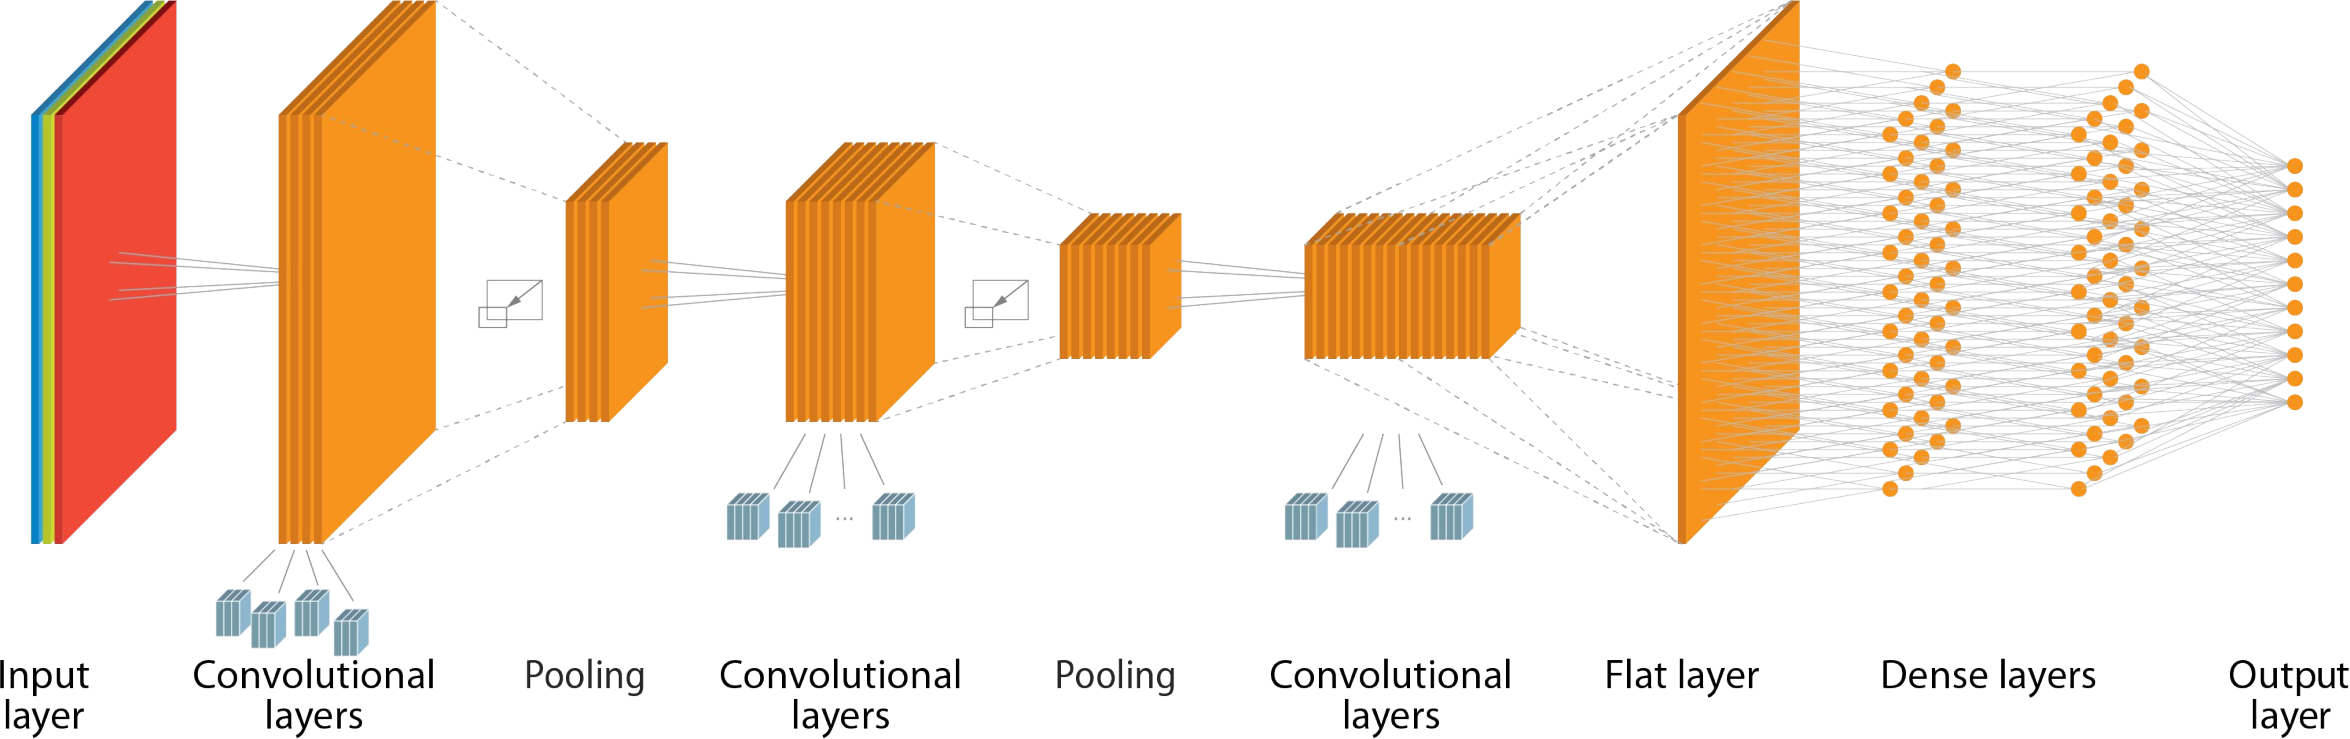
\includegraphics[width=\textwidth]{img/CNN.png}
    \end{center}
  \end{textblock}
\end{frame}

\begin{frame}
  \frametitle{\acl{CNN}: Convolutions}

  \begin{textblock}{90}(5,10)
    \begin{center}
      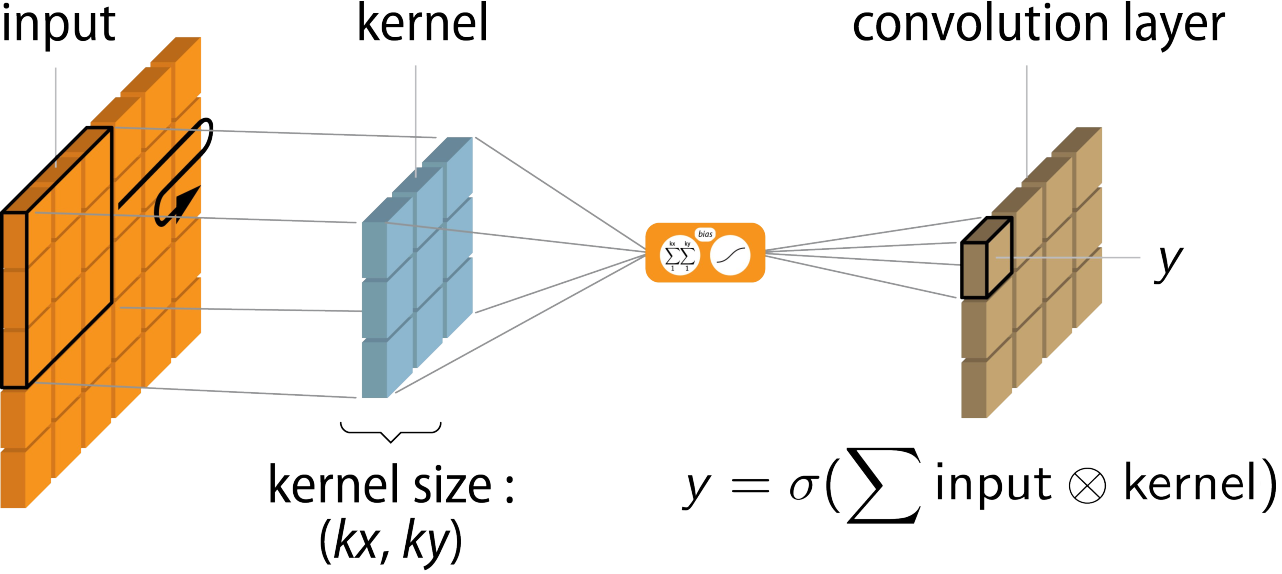
\includegraphics[width=\textwidth]{img/Convolution.png}
    \end{center}
  \end{textblock}
\end{frame}


\begin{frame}
  \frametitle{What have we learned so far?}

  \begin{itemize}
  \item No magic!
  \item A bit of Neural Networks:
    \begin{itemize}
    \item Neurons: activation function
    \item Architecture: layers and weights
    \item Learning: back-propagation
    \end{itemize}
  \item Neural networks are very flexible:
    \begin{itemize}
    \item Universal approximation theorem(s)
    \item Mathematical foundations are not great, not terrible
    \end{itemize}
  \item ML is not only about training models:
    \begin{itemize}
    \item Need a lot of data \& computational power
    \end{itemize}
  \item Data hell
  \end{itemize}
\end{frame}
